\chapter{Post-Processing techniques for current density calculation}
\chaptermark{Current density evaluation}
\label{chap: postprocess}

In many physical and engineering problems the real interesting variable of the conservation law is the flux inside the domain. The study of micro and nano electronics devices does not except this observation so that an accurate description of the current density is a basic requirement.
However, we recall that we chose to follow a displacement approach and this implies that the current density is not a dependent variable of the system but rather a post-calculated quantity.

In this chapter we present the standard Drift-Diffusion formula and we propose an extension of the 1D Scharfetter-Gummel scheme \cite{Gummel:SignAnalys} to the 3D case through two novel schemes:
\begin{itemize}
\item[-] \textit{edge average approximation};
\item[-] \textit{alternative upwinding technique}.   
\end{itemize}

The results obtained are compared with a well tested field simulator as a reference (SDEVICE).

\section{Drift-Diffusion formula}

In Section \ref{sec: carrier transport} we have presented three different but mathematically equivalent ways to represent the current density, but not all of them are appropriate for numerical implementation. In particular we exluded from our analysis the \textit{Slotboom equations} \referenzaeq{eq: Jn slotboom}-\referenzaeq{eq: Jp slotboom} because  the exponential dependency by the factor $\varphi / V_{th}$ brings unavoidable numerical instability. 
The classical \textit{Drift-Diffusion formula} \referenzaeq{eq: drift diff electron}-\referenzaeq{eq: drift diff hole} presents also some difficulties: the drift and diffusion contributions are respectively well defined but the combination of them may give rise oscillations.

Let us introduce some useful notation: with the subscript $K$  we refer to a quantity defined on elements, while the subscript $h$ refers to a quantity defined on vertices. The solutions $\varphi_h$, $n_h$ and $p_h$ obtained with the discretization scheme presented in Section \ref{sec: Numerical approximation} are piecewise linear continuous functions over $\mathcal{T}_h$. According to  \referenzaeq{eq: drift diff electron} and \referenzaeq{eq: drift diff hole},  in order to compute $\vect{J}_n$ and $\vect{J}_p$ numerical differentiation of the solutions must be carried out. Notice that $\vect{J}_{n},\vect{J}_{p} \in [X_h^0]^3$. If we want combine solutions and their derivatives, we have to compute appropriate projection of $n_h$ and $p_h$
 
 \begin{align*}
 n|_K := <n_h> \\ 
p|_K := <p_h>
 \end{align*}
where with the symbol $<\cdot >$ we refer to a suitable average on the element, as presented in Section \ref{sec: continuity equations}. If the diffusion and the mobility coefficients are variable functions of the space and defined on vertices they also have to be projected on the space $X_h^0$.

We implemented a numerical differentiation based on Lagrange polynomial interpolation

\begin{align*}
\nabla n \simeq \nabla (\Pi^1_h n) & = \sum_{i=1}^{N_h} n_i \nabla \psi_i = \nabla n_h \\
\nabla p \simeq \nabla (\Pi^1_h p) & = \sum_{i=1}^{N_h} p_i \nabla \psi_i = \nabla p_h
\end{align*}
 
Notice that $\nabla n_h, \, \nabla p_h \in X_h^0$.
The discretized form of equations \referenzaeq{eq: Jn DD}, \referenzaeq{eq: Jp DD} reads as:

\begin{align}
\vect{J}_n|_K &= -qn|_K\mu_n\nabla \varphi_h + qD_n n|_K\nabla n_h \label{eq: Jn DD discrete}\\ 
\vect{J}_p|_K &= -qp|_K\mu_p\nabla \varphi_h - qD_p p|_K \nabla p_h \label{eq: Jp DD discrete} 
\end{align}
where for sake of simplicity we assume constant diffusion and mobility coefficients in $K$.
Equations \referenzaeq{eq: Jn DD discrete} and \referenzaeq{eq: Jp DD discrete} can be easily computed over each element of $\mathcal{T}_h$.

%  \referenzaeq{eq: Jn qf} and \referenzaeq{eq: Jp qf}
%\vect{J}_n^k &= -q<n>\mu_n\nabla \varphi_n \label{eq: Jn qf discrete}\\
%\vect{J}_p^k &= -q<p>\mu_p\nabla \varphi_p \label{eq: Jp qf discrete} 
% \textcolor{red}{Aggiungere figure dei contributi drift a diffusion separati e del bilancio oscillante per un caso semplice come il diodo. Aggiungere inoltre un caso con il MOS n-channel che verr\`a confrontato con le modifiche apportate dalla formula nella sezione upwinding.}
%\begin{figure}[!h]
%\centering
%
%\subfloat[][\emph{Jn}]
%{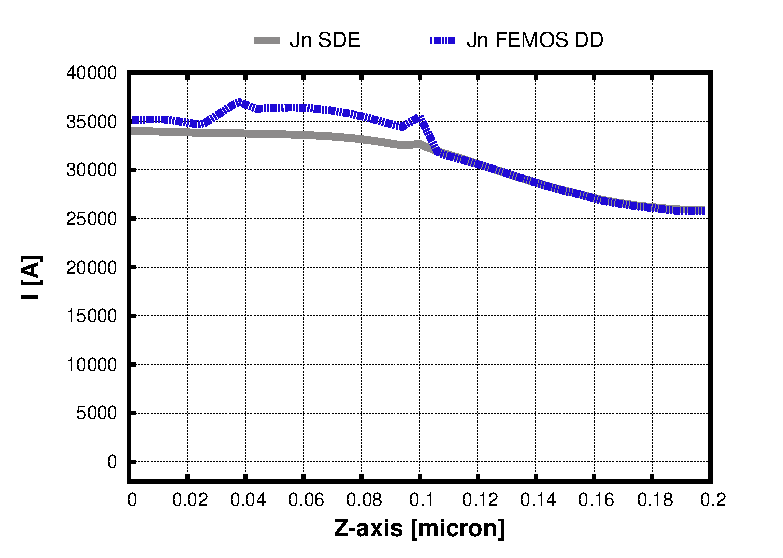
\includegraphics[height=4.5cm]{Corrente/ConfrontiCorrentiBulkJN_SDEVsDD.eps}}
%\subfloat[][\emph{Jp}]
%{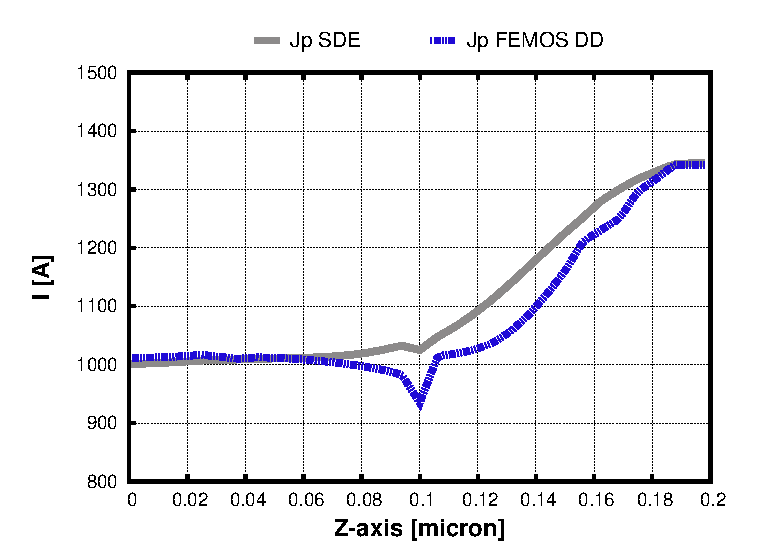
\includegraphics[height=4.5cm]{Corrente/ConfrontiCorrentiBulkJP_SDEVsDD.eps}}
%
%\subfloat[][\emph{Jn}]
%{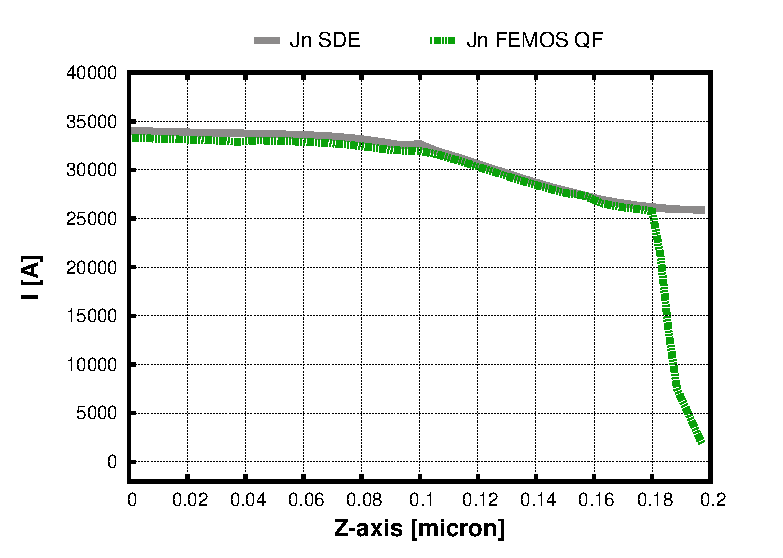
\includegraphics[height=4.5cm]{Corrente/ConfrontiCorrentiBulkJN_SDEVsQF.eps}}
%\subfloat[][\emph{Jp}]
%{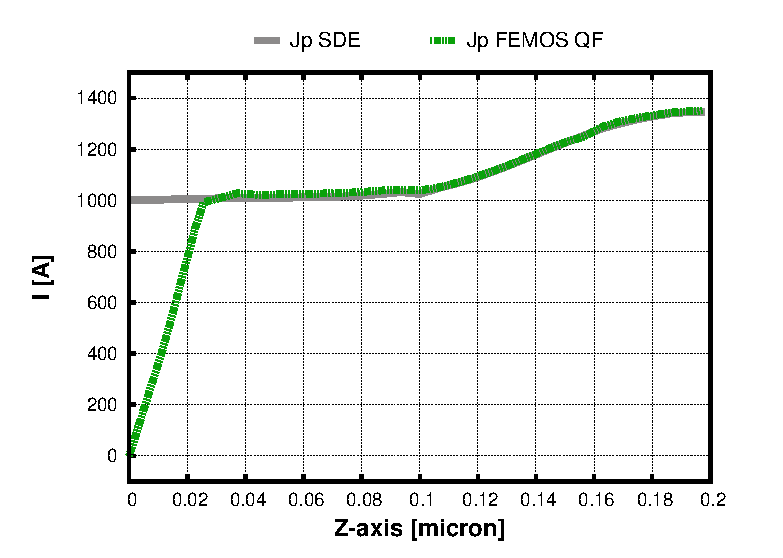
\includegraphics[height=4.5cm]{Corrente/ConfrontiCorrentiBulkJP_SDEVsQF.eps}}
%
%
%\end{figure} 
 

%\begin{figure}[!h]
%\centering
%
%\subfloat[][\emph{Jn}]
%{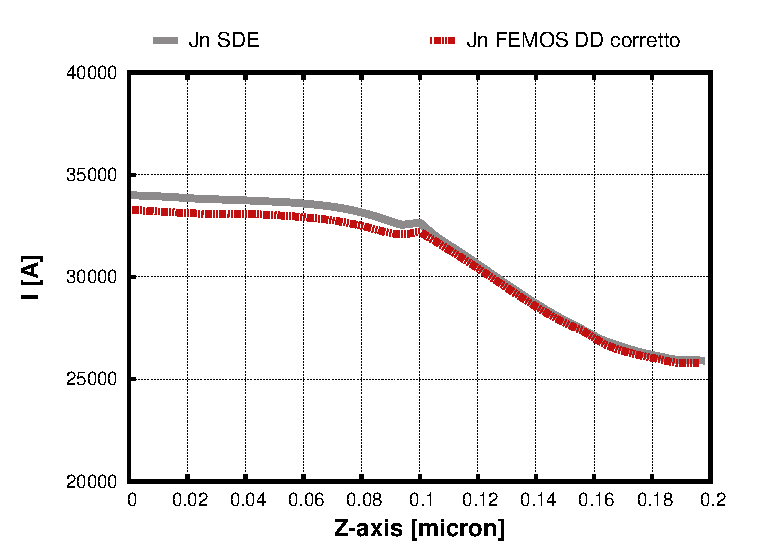
\includegraphics[height=4.5cm]{Corrente/ConfrontiCorrentiBulkJN_SDEVsDDcorretto.eps}}
%\subfloat[][\emph{Jp}]
%{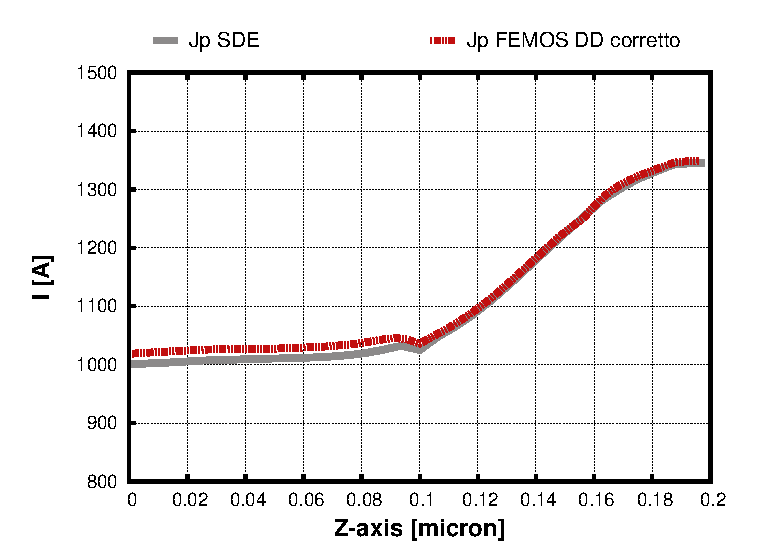
\includegraphics[height=4.5cm]{Corrente/ConfrontiCorrentiBulkJP_SDEVsDDcorretto.eps}}
%
%\subfloat[][\emph{Jn}]
%{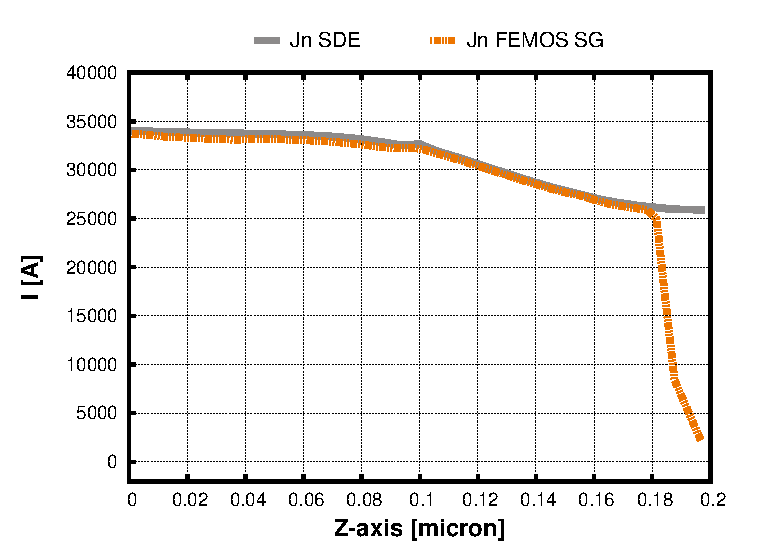
\includegraphics[height=4.5cm]{Corrente/ConfrontiCorrentiBulkJN_SDEVsSG.eps}}
%\subfloat[][\emph{Jp}]
%{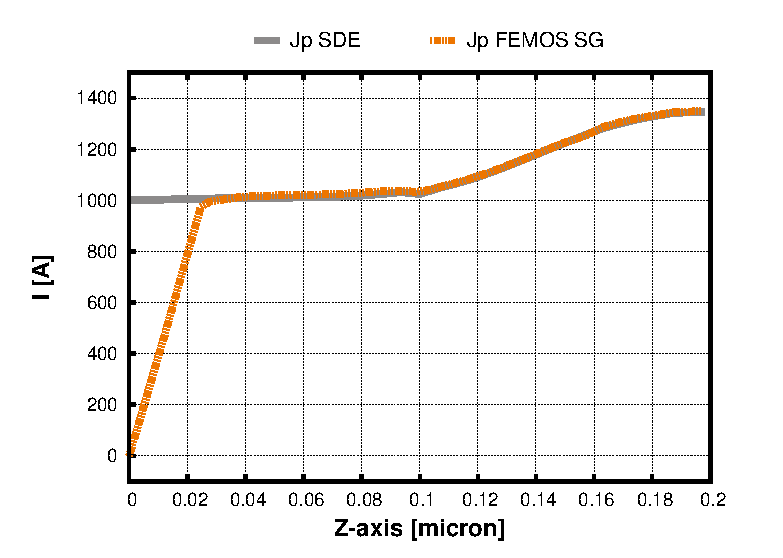
\includegraphics[height=4.5cm]{Corrente/ConfrontiCorrentiBulkJP_SDEVsSG.eps}}
%
%
%\end{figure} 

 
 
\section{Edge averaging techniques} 
 
It is well known that the classical Scharfetter-Gummel (SG) scheme for discretizing drift-diffusion models has proven to be the workhorse for semiconductor device modeling codes \cite{Gummel:SignAnalys}. As a matter of fact the EAFE scheme proposed in Section \ref{sec: continuity equations} is strictly related to the FVSG (Finite Volume Scharfetter-Gummel) method presented by Bank, Fichtner and Rose \cite{Bank:FVSG}. 

In this section we recall the Scharfetter-Gummel formula in a one-dimension spatial domain and we report the extension of the method to the 2D case proposed in \cite{Bank:FEvsBOX}. Finally we present a novel method in order to extend the Scharfetter-Gummel approach to the 3D framework.

\subsection{The 1D Scharfetter-Gummel scheme}

Consider the solution of the electron continuity equation along a one-dimensional domain. For sake of simplicity, we assume a uniform partition. Moreover at every node is defined $\varphi_h$, and in every element the associated electrostatic field $\vect{E}_K$.

 In 1969 D. Scharfetter and H.K. Gummel (two scientists of Bell Labs), introduced a formula to compute the current densities given $\varphi_h$ and $n_h$, $p_h$ at each node of the discretization grid. 
 
The constitutive law for the current density is composed by a drift component, which depends on the electric field, and a diffusion component, which depends on the variation of the carrier density. Consider the geometry shown in \figref{fig: SF figure}, given a generic element $K$ and define the voltage drop $\Delta \varphi|_K=\varphi_{i+1}-\varphi_{i}$ we can distinguish three limit situations: 
\begin{itemize}
\item $\Delta \varphi|_K \gg0$, mainly drift component from right to left 
\item $\Delta \varphi|_K \ll0$, mainly drift component from left to right
\item $\Delta \varphi|_K \simeq 0$, mainly diffusion component
\end{itemize} 
 
 
\begin{figure}[!h]
\centering
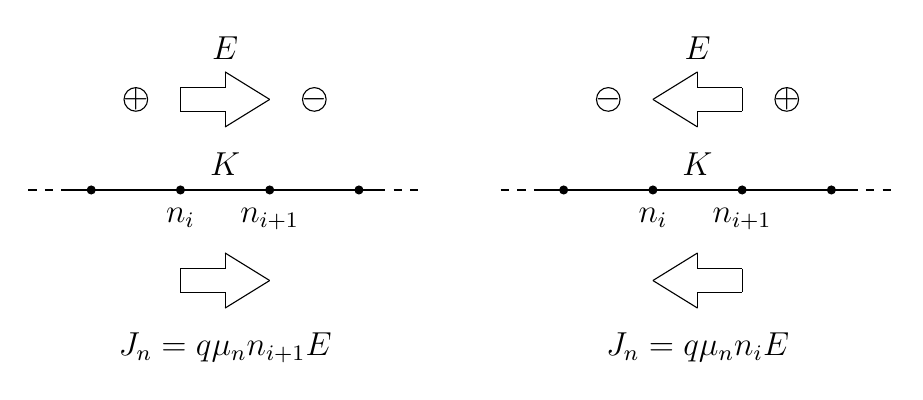
\begin{tikzpicture}
[scale=1.0]
%Solid line
\def\ax{0.5}
\def\ay{0}
\def\bx{4.5}
\def\by{0}

\def\delta{0.3}

%Dash line
\def\cx{0}
\def\cy{0}
\def\dx{5}
\def\dy{0}

\def\Np{3}
\def\step{\bx/\Np-\ax/\Np-2*\delta/\Np}
\def\halfstep{0.5*\bx/\Np-0.5*\ax/\Np-\delta/\Np}

\draw [dashed] (\cx,\cy)--(\dx,\dy);
\draw [thick](\ax,\ay)--(\bx,\by);

\draw [black,draw, fill=black] (\ax+\delta,\ay) circle [radius=0.05];
\draw [black,draw, fill=black] (\ax+\delta+\step,\ay) circle [radius=0.05];
\draw [black,draw, fill=black] (\ax+\delta+\step+\step,\ay) circle [radius=0.05];
\draw [black,draw, fill=black] (\ax+\delta+\step+\step+\step,\ay) circle [radius=0.05];

\draw [thick] (\ax+\delta +\step+\halfstep,\ay+0.05) node[above]{\large $K$};
\draw [thick] (\ax+\delta+\step,\ay-0.1) node[below]{\large $n_{i}$};
\draw [thick] (\ax+\delta+\step + \step,\ay-0.1) node[below]{\large $n_{i+1}$};


\draw [black,draw] (\ax+\delta+\halfstep,\ay+1.15) circle [radius=0.15];
\draw [black,draw] (\ax+\delta+\step + \step + \halfstep,\ay+1.15) circle [radius=0.15];
\node at (\ax+\delta + \halfstep,\ay+1.15){\large $+$};
\node at (\ax+\delta +\step + \step + \halfstep,\ay+1.15){\large $-$};

\node at (\ax+\delta +\step + \halfstep,\ay+1.8){\large $\vect{E}$};
\node at (\ax+\delta +\step + \halfstep,\ay-2.0){\large $\vect{J}_n=q\mu_n n_{i+1}\vect{E}$};

%Freccia
\draw (\ax+ \delta + \step,\ay+1)--(\ax+\delta+\step+\halfstep,\ay+1);
\draw (\ax+\delta + \step,\ay+1.3)--(\ax+\delta+\step+\halfstep,\ay+1.3);
\draw (\ax+\delta+ \step,\ay+1)--(\ax+\delta+\step,\ay+1.3);
\draw (\ax+\delta + \step +\halfstep,\ay+1.3)--(\ax+\delta+\step+\halfstep,\ay+1.5);
\draw (\ax+\delta + \step +\halfstep,\ay+1)--(\ax+\delta+\step+\halfstep,\ay+0.8);
\draw (\ax+\delta + \step +\halfstep,\ay+1.5)--(\ax+\delta+\step+\step,\ay+1.15);
\draw (\ax+\delta + \step +\halfstep,\ay+0.8)--(\ax+\delta+\step+\step,\ay+1.15);

%Freccia
\draw (\ax+ \delta + \step,\ay-1)--(\ax+\delta+\step+\halfstep,\ay-1);
\draw (\ax+\delta + \step,\ay-1.3)--(\ax+\delta+\step+\halfstep,\ay-1.3);
\draw (\ax+\delta+ \step,\ay-1)--(\ax+\delta+\step,\ay-1.3);
\draw (\ax+\delta + \step +\halfstep,\ay-1.3)--(\ax+\delta+\step+\halfstep,\ay-1.5);
\draw (\ax+\delta + \step +\halfstep,\ay-1)--(\ax+\delta+\step+\halfstep,\ay-0.8);
\draw (\ax+\delta + \step +\halfstep,\ay-1.5)--(\ax+\delta+\step+\step,\ay-1.15);
\draw (\ax+\delta + \step +\halfstep,\ay-0.8)--(\ax+\delta+\step+\step,\ay-1.15);



%Solid line
\def\ax{6.5}
\def\ay{0}
\def\bx{10.5}
\def\by{0}

\def\delta{0.3}

%Dash line
\def\cx{6}
\def\cy{0}
\def\dx{11}
\def\dy{0}

\def\Np{3}
\def\step{\bx/\Np-\ax/\Np-2*\delta/\Np}
\def\halfstep{0.5*\bx/\Np-0.5*\ax/\Np-\delta/\Np}

\draw [dashed] (\cx,\cy)--(\dx,\dy);
\draw [thick](\ax,\ay)--(\bx,\by);

\draw [black,draw, fill=black] (\ax+\delta,\ay) circle [radius=0.05];
\draw [black,draw, fill=black] (\ax+\delta+\step,\ay) circle [radius=0.05];
\draw [black,draw, fill=black] (\ax+\delta+\step+\step,\ay) circle [radius=0.05];
\draw [black,draw, fill=black] (\ax+\delta+\step+\step+\step,\ay) circle [radius=0.05];

\draw [thick] (\ax+\delta +\step+\halfstep,\ay+0.05) node[above]{\large $K$};
\draw [thick] (\ax+\delta+\step,\ay-0.1) node[below]{\large $n_{i}$};
\draw [thick] (\ax+\delta+\step + \step,\ay-0.1) node[below]{\large $n_{i+1}$};

\draw [black,draw] (\ax+\delta+\halfstep,\ay+1.15) circle [radius=0.15];
\draw [black,draw] (\ax+\delta+\step + \step + \halfstep,\ay+1.15) circle [radius=0.15];
\node at (\ax+\delta + \halfstep,\ay+1.15){\large $-$};
\node at (\ax+\delta +\step + \step + \halfstep,\ay+1.15){\large $+$};

\node at (\ax+\delta +\step + \halfstep,\ay+1.8){\large $\vect{E}$};
\node at (\ax+\delta +\step + \halfstep,\ay-2.0){\large $\vect{J}_n=q\mu_n n_{i}\vect{E}$};


%Freccia
\draw (\ax+ \delta + \step +\halfstep,\ay+1)--(\ax+\delta+\step +\step,\ay+1);
\draw (\ax+\delta + \step + \halfstep,\ay+1.3)--(\ax+\delta+\step + \step,\ay+1.3);
\draw (\ax+\delta+ \step + \step,\ay+1)--(\ax+\delta+\step+\step,\ay+1.3);
\draw (\ax+\delta + \step +\halfstep,\ay+1.3)--(\ax+\delta+\step+\halfstep,\ay+1.5);
\draw (\ax+\delta + \step +\halfstep,\ay+1)--(\ax+\delta+\step+\halfstep,\ay+0.8);
\draw (\ax+\delta + \step +\halfstep,\ay+1.5)--(\ax+\delta+\step,\ay+1.15);
\draw (\ax+\delta + \step +\halfstep,\ay+0.8)--(\ax+\delta+\step,\ay+1.15);

%Freccia
\draw (\ax+ \delta + \step +\halfstep,\ay-1)--(\ax+\delta+\step +\step,\ay-1);
\draw (\ax+\delta + \step + \halfstep,\ay-1.3)--(\ax+\delta+\step + \step,\ay-1.3);
\draw (\ax+\delta+ \step + \step,\ay-1)--(\ax+\delta+\step+\step,\ay-1.3);

\draw (\ax+\delta + \step +\halfstep,\ay-1.3)--(\ax+\delta+\step+\halfstep,\ay-1.5);
\draw (\ax+\delta + \step +\halfstep,\ay-1)--(\ax+\delta+\step+\halfstep,\ay-0.8);
\draw (\ax+\delta + \step +\halfstep,\ay-1.5)--(\ax+\delta+\step,\ay-1.15);
\draw (\ax+\delta + \step +\halfstep,\ay-0.8)--(\ax+\delta+\step,\ay-1.15);

\end{tikzpicture}

\caption{Effect of a high electric field over the current density of electron.}
\label{fig: SF figure}
\end{figure}

All these situations can be accounted for by the following unifying formula

 \begin{equation}
\label{eq: scharfetter gummel 1D electron}
J_n|_K=q\frac{D_n}{h}
\left[ n_{i+1}\mathcal{B}\left(\frac{\Delta \varphi|_K}{V_{th}}\right)- n_i\mathcal{B}\left(-\frac{\Delta \varphi|_K}{V_{th}}\right)\right].  
\end{equation}

In the case $\Delta \varphi|_K=0$, the SG formula becomes

\begin{equation}
J_n|_K=qD_n\frac{n_{i+1}-n_{i}}{h}
\end{equation}
which is the correct approximation of the current density using a $\mathbb{P}_1$ basis for $n_h$. When $\Delta \varphi|_K \gg 0$, the SG formula becomes

\begin{equation}
J_n|_K = q\mu_n n_{i}\dfrac{\Delta \varphi|_K}{h}
\end{equation}
while for $\Delta \varphi|_K \ll 0$ we have

\begin{equation}
J_n|_K = q\mu_n n_{i+1}\dfrac{\Delta \varphi|_K}{h}.
\end{equation}

The current density on the element $K$ becomes similar to the Ohm's law where the carrier transported is $n_{i+1}$ when $\Delta \varphi|_K \ll 0$ or $n_i$ when $\Delta \varphi|_K \gg 0$. These situations are well illustreated in \figref{fig: SF figure}.
Analogous considerations holds also for the holes, considering the associated formula for the current density

 \begin{equation}
\label{eq: scharfetter gummel 1D hole}
J_p|_K=q\frac{D_p}{h}
\left[ p_{i+1}\mathcal{B}\left(-\frac{\Delta \varphi|_K}{V_{th}}\right)- p_i\mathcal{B}\left(\frac{\Delta \varphi|_K}{V_{th}}\right)\right].  
\end{equation}


\subsection{The 2D Scharfetter-Gummel scheme}

One of the main results of \cite{Bank:FEvsBOX} is the equivalence between the finite volume approach and the finite element Galerkin discretizations of the continuity equation. In order to facilitate the connection between these two different discretization approaches the authors introduce for each $K \in \mathcal{T}_h$ a linear map $\mathcal{J}_{K}:\mathbb{R}^3\rightarrow\mathbb{R}^2$ defined by

\begin{equation}
\label{eq: map current}
\mathcal{J}_{K}(\{\gamma_i\}_{i=1}^3) = \dfrac{1}{|K|}\sum_{i=1}^3 \gamma_i |e_i| s_i \vect{t}_i
\end{equation}
where $s_i$ is the meausure of the segment from the midpoint  of $e_i$ to the intersection of the perpendicular edge bisectors and $\vect{t}_i$ denotes the unit tangent vector of the edge $e_i$ (see \figref{fig: parameter 2D}).
$\mathcal{J}_K$ has the following properties:

\begin{align}
\mathcal{J}_K(\{\vect{J}\cdot \vect{t}_i\}_{i=1}^3) & = \vect{J} \label{eq: map is current} \\
 \mathcal{J}_K(\{s_i^{-1}\}_{i=1}^3) & = 0 \\
 \int_K \mathcal{J}_K(\{\gamma_i\}_{i=1}^3) \cdot \nabla \psi \, dK & = \gamma_{i+1}s_{i+1} - \gamma_{i-1}s_{i-1}.
\end{align}
 
Equation \referenzaeq{eq: map is current} says that if we are able to compute the tangential component of the current density over all edges, we can combine these values according to \referenzaeq{eq: map current} and obtain the current density $\forall K \in \mathcal{T}_h$.
 
Using the EAFE scheme, in the case of electron we have
 
\begin{equation}
\label{eq: EAFE edge formula}
\small
\vect{J}_n\cdot \vect{t}_i = qD_n  \dfrac{\mathcal{B}(\delta_i(\varphi_h / V_{th}))n_{h,k} -  \mathcal{B}(-\delta_i(\varphi_h / V_{th}))n_{h,j}}{|e_i|}
\end{equation}
where 

\begin{equation}
\delta_i(\varphi_h/V_{th}) = \dfrac{\varphi_{h,k}-\varphi_{h,j}}{V_{th}}.
\end{equation}

%Similarly for the classical FVSG scheme this contribution is defined as
%
%\begin{equation}
%\vect{J}_n\cdot \vect{t}_i = \mathcal{H}_{e_i}(qD_n e^{\varphi_h/V_{th}}) \nabla (\Pi^1|_K(e^{-\varphi_h / V_{th}}n_h)) \cdot \vect{t}_i
%\end{equation}
%where $\mathcal{H}_{e_i}$ is the harmonic average along the edge $e_i$ and $\Pi^1|_K$ is the interpolant over $K$.
The extension of this procedure to the 3D case is non trivial, because the characterization of the cross-section $s_i$ becomes much more complex.

\begin{figure}[!h]
\centering
\begin{tikzpicture}
% Vertici del triangolo
\coordinate [label=below left:$v_2$]			(A) at (0,0);
\coordinate [label = $v_1$]							(B) at (4,4);
\coordinate [label =below right:$v_3$]		(C) at (6,0);
% Punti medi
\coordinate [label=above right:$e_2$]					(Ap) at ($(B)!	0.5!(C)$);
\coordinate [label=below:$e_1$]  				(Bp) at ($(A)!0.5!(C)$);
\coordinate [label=above left:$e_3$]					(Cp) at ($(A)!0.5!(B)$);
% Piedi delle altezze
%\coordinate [label=45:$A’’$]  				(As) at ($(B)!(A)!(C)$);
%\coordinate [label=-90:$B’’$] 				(Bs) at ($(A)!(B)!(C)$);
%\coordinate [label=180:$C’’$] 			(Cs) at ($(A)!(C)!(B)$);

% Circocentro
\coordinate []						(Ca) at ($(Ap)!1!90:(B)$);
\coordinate []						(Cb) at ($(Bp)!0.34!90:(C)$);
\coordinate []						(Cc) at ($(Cp)!0.5!90:(A)$);
% Punti medi C
\coordinate [label=above left:$s_2$]				(Cap) at ($(Ap)!	0.5!(Ca)$);
\coordinate [label=right:$s_1$]  			(Cbp) at ($(Bp)!0.5!(Cb)$);
\coordinate [label=below left:$s_3$]				(Ccp) at ($(Cp)!0.5!(Cc)$);
% Punti per tangenti
\coordinate [label=below right:$\mathbf{t}_1$]				(ta) at ($(A)!0.2!(C)$);
\coordinate [label=above right:$\mathbf{t}_2$]  			(tb) at ($(C)!0.2!(B)$);
\coordinate [label=above left:$\mathbf{t}_3$]				(tc) at ($(B)!0.2!(A)$);


% Disegno del triangolo, mediane e altezze
%\draw [red] (A) -- (Ap) (B) -- (Bp) (C) -- (Cp);
\draw [] (Ca) -- (Ap) (Cb) -- (Bp) (Cc) -- (Cp);
\draw [->,ultra thick] (A) -- (ta) ;
\draw [->,ultra thick] (C) -- (tb) ;
\draw [->, ultra thick] (B) -- (tc);
%\draw [blue, dashed]
  %    (A) -- (As) (B) -- (Bs) (C) -- (Cs);
\draw [thick] (A) -- (B) -- (C) -- cycle ;
\end{tikzpicture}
\caption{Parameters associated with element $K$ for the current density calculation.}
\label{fig: parameter 2D}
\end{figure}

\subsection{The 3D Scharfetter-Gummel scheme}
\label{sec: SG 3D} 
 
In this section we present novel method for the reconstruction of the electron current density over each element of the grid that is based on the so-called Primal-Mixed formulation \cite{Roberts:MixedHybrid}.

We start by recalling here the formula for the electron current density expressed as a function of the quasi Fermi potential

\begin{equation}
\label{eq: current density fermi}
\vect{J}_n=-q \mu_n n \nabla \varphi_n.
\end{equation}

Relation \referenzaeq{eq: current density fermi} can be written considering equation \referenzaeq{eq: non eq n density mb} as

\begin{equation}
\label{eq: current density canonic form}
\vect{J}_n\dfrac{ \exp\left(\dfrac{\varphi_n-\varphi}{V_{th}}\right)}{q \mu_n n_i} + \nabla \varphi_n = 0.
\end{equation}

Let $\vect{J}_n\in[L^2(\Omega)]^3$ and $\varphi_n,\varphi \in H^1(\Omega)$. We multiply \referenzaeq{eq: current density canonic form} with a generic function $\vect{q}\in[L^2(\Omega)]^3$ and then intagrate over the domain $\Omega$:

\begin{equation}
\label{eq: variation form of current density continuos}
\int_\Omega \dfrac{ \exp \left( \dfrac{\varphi_n-\varphi}{V_{th}} \right) }{q \mu_n n_i} \vect{J}_n \cdot \vect{q} \, d\Omega
 + \int_\Omega \nabla \varphi_n \cdot \vect{q} \, d\Omega = 0 
\end{equation}


We proceed using the discrete space of the piecewise constant functions over $\mathcal{T}_h$

\begin{equation}
\label{eq: spaces elementwise constant}
V_h=\left\{ w \in L^2(\Omega) : w|_{K}\in \mathbb{P}_0 \forall K \in \tau_h\right\}.
\end{equation}

Now the discrete quantities are $\vect{J}_n^h\in[V_h]^3$ and $\nabla \varphi_n^h \in V_h$. We consider the following choice of the test function $\vect{q}_h \in [V_h]^3$

\begin{equation}
\label{eq: form of qh}
\vect{q}^h_{1,2,3} = \left\{ \begin{bmatrix} 1 \\ 0 \\ 0 \end{bmatrix}  \begin{bmatrix} 0 \\ 1 \\ 0 \end{bmatrix}  \begin{bmatrix} 0 \\ 0 \\ 1 \end{bmatrix}  \right\}.
\end{equation}

From \referenzaeq{eq: variation form of current density continuos} we obtain a system of equations defined for each $K \in \mathcal{T}_h$:

\begin{equation}
\label{eq: variation form of current density}
\int_K \dfrac{ \exp \left( \dfrac{\varphi_n-\varphi}{V_{th}} \right) }{q \mu_n n_i} \vect{J}_n^h \cdot \vect{q}^h_i \, dK
 + \int_K \nabla \varphi_n^h \cdot \vect{q}^h_i \, dK = 0 \psp{10}  i=1,2,3
\end{equation}

After integration we have for the generic component of the current density

\begin{equation}
\label{eq: first formula for J}
[\vect{J_n}]_i = - \mathcal{H}_K \left( q \mu_n n_i \exp \left( \dfrac{\varphi-\varphi_n}{V_{th}} \right)  \right) \dfrac{\partial \varphi_n^h}{\partial x_i} \psp{5} i = 1,2,3, \psp{5} \forall K \in \tau_h
\end{equation}

We do not evaluate the harmonic average with an exact 3D integration because it may be computationally expensive. Therefore, we approximate $\mathcal{H}_K(\cdot)$ by the following quadrature

\begin{equation}
\label{eq: approzimation from 3D to edge}
\left(\dfrac{\int_K f^{-1} \, dK}{|K|} \right)^{-1} \simeq \left(\dfrac{\int_{e*} f^{-1} \, de}{|e^*|} \right)^{-1}
\end{equation}
 where 
\begin{equation*}
 f=q \mu_n n_i exp((\varphi-\varphi_n)/V_{th}) \, ,
\end{equation*} 
 and $e^*$ is the edge of $\partial K$ where the maximum drop of $f$ occuring.
This becomes by the fact that the diffusion coefficient is represented by the edge where the phenomenon are more significant rather than considering the entire element: the problem now is the indentification of the correct edge. Let us consider a quantity defined at the vertices

\begin{equation}
\label{eq: differenza tra pot e qf}
\Phi := \dfrac{\varphi - 	\varphi_n}{V_{th}}
\end{equation}
which is the difference between the electrostatic potential and the quasi Fermi potential level. Now for every element consider two vertices: $\vect{x}_m$ s.t. $\Phi(\vect{x}_m)=\Phi_m := \min_K(\Phi)$ and $\vect{x}_M$ s.t. $\Phi(\vect{x}_M)=\Phi_M:=\max_K(\Phi)$. Obviously it exists only one edge which connects these two points and on this one we perform the 1D integration \referenzaeq{eq: approzimation from 3D to edge}.

%\begin{equation}
%\left(\dfrac{1}{|e^*|} \int_{e*} \dfrac{   exp \left( %\dfrac{\varphi_n-\varphi}{V_{th}} \right) }{ q \mu_n n_i} \, de %\right)^{-1}
%\end{equation}


Along the edge $e^*$ we have

\begin{equation}
f(s) = q \mu_n n_i \exp\left( \Phi_m + (\Phi_M-\Phi_m)\dfrac{s-s_m}{|e^*|} \right)
\end{equation}

where $s \in [s_m,s_M]$ is the parameter refered to the edge $e^*$ s.t. $f(s_m)=f(\vect{x}_m)$ and $f(s_M)=f(\vect{x}_M)$. We can solve \referenzaeq{eq: approzimation from 3D to edge} with the following change of variables $\eta := (s-s_m)/|e^*|$ and proceed with trivial integration steps, to obtain

\begin{align*}
\int_{e^*} f^{-1} \, de & = |e^*| \int_0^1 \dfrac{\exp \left(-\Phi_m - (\Phi_M-\Phi_m)\eta \right)}{q\mu_n n_i} 
 \, d\eta \\
  & = |e^*|\dfrac{\exp (-\Phi_m)}{q\mu_n n_i} \dfrac{\exp ( \Phi_m-\Phi_M)-1}{\Phi_m-\Phi_M} \\
 & =  |e^*|\dfrac{\exp (-\Phi_m)}{q\mu_n n_i} \dfrac{1}{\mathcal{B}(\Phi_m-\Phi_M)}
\end{align*}
from which we finally get

\begin{equation}
\label{eq: finally approzimation 3D to 1D}
\int_{K} f^{-1} \, dK \simeq  q \mu_n n_i \exp(\Phi_m) \mathcal{B}(\Phi_m-\Phi_M).
\end{equation}

Similar results may be obtained repeating the integration and considering $s_M$ as starting point

\begin{equation}
\label{eq: approssimazione sm}
\int_{K} f^{-1} \, dK \simeq  q \mu_n n_i \exp(\Phi_M) \mathcal{B}(\Phi_M-\Phi_m).
\end{equation}

Equation \referenzaeq{eq: finally approzimation 3D to 1D} and \referenzaeq{eq: approssimazione sm} can be combined to find

\begin{equation}
\label{eq: first formula for J}
\vect{J}_n|_K = -  q \mu_n  \left[ \dfrac{ n_{\min} \mathcal{B}(-\Delta \Phi_{max})  + n_{\max}\mathcal{B}(\Delta \Phi_{max})}{2} \right]\nabla \varphi_n^h
\end{equation}
where $n_{\min}=n_i e^{\Phi_m}$ and $n_{\max}=n_i e^{\Phi_M}$ while $\Delta \Phi_{\max} := \Phi_M - \Phi_m$. If we consider equation \referenzaeq{eq: first formula for J} over a one-dimensional domain we can recover equation \referenzaeq{eq: scharfetter gummel 1D electron}, which shows that the above described approach is the natural extension of the $Scharfetter-Gummel$ formula to the 3D case.
Following the same procedure we obtain for the hole current density
\begin{equation}
\label{eq: first formula for Jp}
\vect{J}_p|_K = -  q \mu_p  \left[ \dfrac{ p_{\min} \mathcal{B}(\Delta \Phi_{max})  + p_{\max}\mathcal{B}(-\Delta \Phi_{max})}{2} \right]\nabla \varphi_p^h
\end{equation}


\section{Upwinding techniques}

It is well known that the classical finite element method applied on a con- vection-diffusion problem is unstable when the solution presents boundary layers. This has led to the introduction of upwinding techniques which in one-dimensional case consists of adding an artificial diffusion term to the origin problem.

% P\`eclet number ($\mathbb{P}e$) is large. The coefficient $\mathbb{P}e$ includes the influence of the drift component and is proportional to the product $|\nabla \varphi| h$. Therefore the presence of boundary layers for the electrostatic potential makes the solution of the continuity equation a difficult task. This has led to the use of upwinding techniques: in the one-dimensional case this consists of adding an artificial diffusion term to the origin convection-diffusion equation.

Using the finite element space $X_h^1$, in the case of the 1D electron continuity equation we have the following perturbed problem

\begin{equation}
\label{eq: perturbed problem}
- \partial_x  (qD_n(1+\Phi(\mathbb{P}e|_K))\partial_x n - q \mu_n n \partial_x \varphi) = -qR.
\end{equation}
where $\Phi$ is the stabilization function and $\mathbb{P}e|_K$ is the local P\`eclet number defined as 
 
 \begin{equation*}
 \mathbb{P}e|_K = \dfrac{\partial_x \varphi_h h}{2V_{th}}  = \dfrac{\Delta \varphi }{2 V_{th}}
 \end{equation*}
 
The weak form associated with problem \referenzaeq{eq: perturbed problem} is

\begin{equation}
\label{eq: weak form perturbed}
a_h(n,v) = a(n,v) + \sum_{K\in \mathcal{T}_h}\int_{K} \Phi(\mathbb{P}e|_K) \partial_x n \cdot \partial_x v \, dK
\end{equation}
and relation \referenzaeq{eq: Jn DD discrete} becomes
\begin{equation}
\label{eq: j element 1d perturbata}
J_n|_K = -qn|_K\mu_n\partial_x \varphi_h + qD_n(1+\Phi(\mathbb{P}e|_K)) n|_K\partial_x n_h .
\end{equation}
where, considering local indices for the vertices of $K$, we have:

\begin{align*}
n|_K & = \dfrac{\int_K n_h \, dx}{|K|} = \dfrac{n_1+n_2}{2} \\
\partial_x \varphi_h & = \dfrac{\varphi_2-\varphi_1}{h} = \dfrac{\Delta \varphi}{h}\\
\partial_x n_h & = \dfrac{n_2 - n_1}{h}.
\end{align*}

In order to guarantee the consistency of \referenzaeq{eq: weak form perturbed} with respect to the standard Galerkin weak form the  stabilization function  must respect the following relation 

\begin{align}
\label{eq: consistenza}
\lim_{\mathbb{P}e|_K \to 0} \Phi(\mathbb{P}e|_K) = 0 \psp{15} \forall K\in\mathcal{T}_h.
\end{align}



%Considering the framework just presented the \textit{Scharfetter-Gummel} discretization scheme in one spatial dimension can be obtained using the following choice of the function $\Phi$
%
%\begin{equation}
%\label{eq: phi per SG 1D}
%\Phi(\mathbb{P}e) = \mathcal{B}(2\mathbb{P}e) + \mathbb{P}e -1
%\end{equation}
The efficiency of an upwinding scheme is related to the choice of $\Phi(\mathbb{P}e|_K)$ and as we are perturbing the problem we would like satisfy some interesting limit cases for the current density formula which occur for the origin problem when we have 
\begin{itemize}
\item[1] \textbf{constant carrier concentrations}
\begin{equation*}
\vect{J}_n  = q\mu_n n \vect{E}\, , \psp{15} \vect{J}_p  = q\mu_p p \vect{E} \, ;
\end{equation*}
\item[2] \textbf{constant potential} ($\vect{E}=0$),
\begin{equation*}
\vect{J}_n  = qD_n\nabla n \, , \psp{15} \vect{J}_p  = -qD_p\nabla p \, ;
\end{equation*}
\item[3] \textbf{constant quasi Fermi potential}, which implies that $n=C_1e^{\varphi / V_{th}}$ and $p=C_2e^{-\varphi / V_{th}}$ where $C_1$ and $C_2$ are two arbitrary constants such that
\begin{equation*}
C_1 = \exp(-\bar\varphi_n/V_{th}) \psp{15} C_2 = \exp(\bar\varphi_p/V_{th})
\end{equation*}
where $\bar\varphi_n$ and $\bar\varphi_p$ are given contact values. Under this assumption from equations \referenzaeq{eq: Jn DD} and \referenzaeq{eq: Jp DD} we have that

\begin{align*}
\vect{J}_n & = -q\mu_n (n\nabla 	\varphi - V_{th} (\dfrac{C_1}{V_{th}}\nabla \varphi e^{\varphi / V_{th}}) = 0\\
\vect{J}_p & = -q\mu_p (p\nabla 	\varphi + V_{th} (-\dfrac{C_1}{V_{th}}\nabla \varphi e^{-\varphi / V_{th}}) = 0
\end{align*}
 
Constant quasi Fermi potentials correspond to thermodynamical equilibrium condition for the carrier densities and implies no current flow in the device.
\end{itemize}

If \referenzaeq{eq: consistenza} occurs relation \referenzaeq{eq: j element 1d perturbata} satisfies case 1 and 2, while case 3 is obtained imposing that

\begin{equation}
J_n|_K(\Pi_1^k(Ce^{\varphi / V_{th}})) = 0 .
\end{equation}

From \referenzaeq{eq: j element 1d perturbata} we have

\begin{align*}
q\mu_n <n_h>\partial_x \varphi_h & = q D_ n(1+\Phi(\mathbb{P}e|_K)\partial_x n_h \\
<n_h>\partial_x \varphi_h & = V_{th}(1+\Phi(\mathbb{P}e|_K))\partial_x n_h \\
\end{align*}
and finally get the following relation for the stabilization function
\begin{equation}
\label{eq: SG stab func alternative}
\Phi(\mathbb{P}e|_K)  = \sigma \mathbb{P}e|_K \dfrac{n_1+n_2}{n_2-n_1}  -1
\end{equation}
where 

\begin{equation*}
\sigma = sign(\Delta \varphi).
\end{equation*}

Now we impose the constant quasi Fermi potential hypothesis

\begin{align*}
\Phi(\mathbb{P}e|_K) & = \sigma \mathbb{P}e|_K \dfrac{e^{\varphi_1/V_{th}}+e^{\varphi_2/V_{th}}}{e^{\varphi_2/V_{th}}-e^{\varphi_1/V_{th}}} -1 \\
& = \sigma \mathbb{P}e|_K \dfrac{e^{\Delta \varphi/V_{th}}+1}{e^{\Delta \varphi/V_{th}}-1} -1 \\
& = \sigma \mathbb{P}e|_K \dfrac{e^{2 \sigma \mathbb{P}e|_K}+1}{e^{2\sigma \mathbb{P}e|_K}-1} -1.
\end{align*}

Setting $X := 2 \sigma \mathbb{P}e|_K$ we have

\begin{align*}
\Phi(X) & = \dfrac{X}{2} \left( \dfrac{e^{X}}{e^{X}-1} + \dfrac{1}{e^{X}-1} \right) -1 \\
& = \dfrac{1}{2} \left( \mathcal{B}(-X) + \mathcal{B}(X) \right) -1 \\
 & = \dfrac{1}{2} \left( X + \mathcal{B}(X) + \mathcal{B}(X) \right) -1 \\
  & =  \mathcal{B}(X) +\dfrac{X}{2}  -1.
\end{align*}

Replacing the definition of $X$ we obtain for both $\Delta \varphi > 0$ and $\Delta \varphi < 0$

\begin{equation}
\label{eq: SG stabilization function}
\Phi(\mathbb{P}e|_K) = \mathcal{B}(2\mathbb{P}e|_K) + \mathbb{P}e|_K -1.
\end{equation}

%Many efforts have been made in order to propose a similar uniform framework  for the study of upwinding schemes also in multidimensional domain \cite{Bank:Upwinding}. 

Considering relation \referenzaeq{eq: SG stabilization function} we obtain the well known 1D Scharfetter-Gummel discretization scheme proposed by Allen and Southwell in \cite{Allen:SGformula}.
In a 3D framework it is not intuitive how to evaluate equation \referenzaeq{eq: SG stabilization function}, but considering  \referenzaeq{eq: SG stab func alternative} we can say that a straightforward extension to the 3D case of the 1D Scharfetter-Gummel stabilization can be found considering a $3\times 3$ diagonal tensor  $\underline{\underline{\vect{\Phi}}}^K$  defined on each element as follows

\begin{equation}
\label{eq: SG stabilized}
\underline{\underline{\vect{\Phi}}}^K_{\, ii} = -\dfrac{<\Pi_1^k(e^{\varphi/V_{th}})> \partial_{x_i}\varphi}{\partial_{x_i}\Pi_1^k(e^{\varphi/V_{th}})V_{th}} -1 \psp{10} i = 1,2,3,
\end{equation}

In \referenzaeq{eq: SG stabilized} the argument of the exponential can be a highly varying function over $K$, therefore it is preferable to consider a reference value for the electrostatic potential.
 Observe that $\varphi \in [\varphi_{min},\varphi_{max}]$ and therefore we can use one of these values as reference and obtain
 
 \begin{equation}
\label{eq: SG stabilized}
\underline{\underline{\vect{\Phi}}}^K_{\, ii}  = -\dfrac{<\Pi_1^k(e^{(\varphi-\varphi_{min})/V_{th}})> \partial_{x_i}\varphi}{\partial_{x_i}\Pi_1^k(e^{(\varphi-\varphi_{min})/V_{th}})V_{th}} -1 \psp{10} i = 1,2,3,
\end{equation}

Finally, for the 3D electron current density we have

\begin{equation}
\vect{J}_n|_K = -qn|_K\mu_n\nabla \varphi_h + qD_nn|_K(\underline{\underline{\mathcal{I}}}+\underline{\underline{\vect{\Phi}}}_K) \nabla n_h.
\end{equation}

where $\underline{\underline{\mathcal{I}}}$ is the $3\times 3$ identity tensor and $n|_K=\mathcal{M}(n_h)$.
\subsection{Results}

In this section we compare the performance of the different current computation methods . The test problems are the p-n junction (\tabref{tab: diode direct}  $V_A=1.0[V]$) and the n-MOSFET (\tabref{tab: mos direct pol} on-state condition).
The procedures considered are:
\begin{itemize}
\item {\bf Drift-Diffusion} defined by \referenzaeq{eq: Jn DD discrete} and \referenzaeq{eq: Jp DD discrete} with $n|_K=\mathcal{M}(n_h)$, where $\mathcal{M}(\cdot)$ is the standard integral average;
\item {\bf Scharfetter-Gummel 3D} method described in section \ref{sec: SG 3D};
\item {\bf Modified Drift-Diffusion} which is for the electron current density 

 and $\underline{\underline{\vect{\Phi}}}_K$ as equation \referenzaeq{eq: SG stabilized}.
\end{itemize}

The comparison currents for the forward biased p-n junction are depicted in \figref{fig: pn current density 1V} using 1D plots along a line parallel to the Z-axis and placed at the center of the device. Both electron and hole current densities are shown for the three methods. 
We note that the best result is obtained by the modified DD method, while the standard DD is unstable and the SG 3D computes wrong values of the current next to the contacts. 
Critical behaviour presented in \figsref{fig: Jn DD} and \ref{fig: Jp DD} are due to the wrong balance between drift and diffusion contributions, this problem is fixed by the upwinding technique as shown in \figsref{fig: Jn DD mod} and \ref{fig: Jp DD mod}.

The SG 3D scheme performs essentially well inside the device but considering the electron current density of \figref{fig: Jn SG 3D} we note incorrect behaviour at the contact where electrons are minority. (\figref{fig: Jp SG 3D} shows the dual effect for the holes). Physically speaking the current densities computed by the SG 3D formula are not wrong, indeed assuming ideal contacts we are enforcing that all the recombination of the excess carriers happens at the contact surface. This phenomena is well depicted by the boundary layers of the hole quasi Fermi potential presented in \figref{fig: QF hole}, moreover we note that as we refine the grid the behaviour is more bounded at contact and as a consequence we obtain a better prediction of $\vect{J}_p$ (\figref{fig: Jp SG 3D finer}).

The results for the n-MOSFET are shown in \figref{fig: nMOSFET current methods} compared with SDEVICE (\figref{fig: SDE n-MOSFET Jn}). The SG 3D scheme performs very well (\figref{fig: SG 3D scheme nMOS}). The most difficulty of the modified Drift-Diffusion scheme is the numerical evaluation of \referenzaeq{eq: SG stabilized}. When the current density presents a mainly component or equation \referenzaeq{eq: SG stabilized} is far from critical computation (zero division or overflow) the upwinding scheme behaves very well. Considering more complex devices the above situations are not more valid and the results obtained are not good (\figref{fig: DD upwind}). A better evaluation of \referenzaeq{eq: SG stabilized} can be recovered using a finer mesh to the detriment of the computational cost. This test is shown in \figref{fig: DD upwind finer} where we use a mesh with $35342$ vertices (about ten times the number of degrees of freedom of the standard mesh). The result is not still good enough but comparing with the standard DD formula \figref{fig: DD standard nMOS} we appreciate a better behaviour.
  
\begin{figure}[!h]
\centering


\subfloat[][\emph{Standard DD - Jn}\label{fig: Jn DD}]
{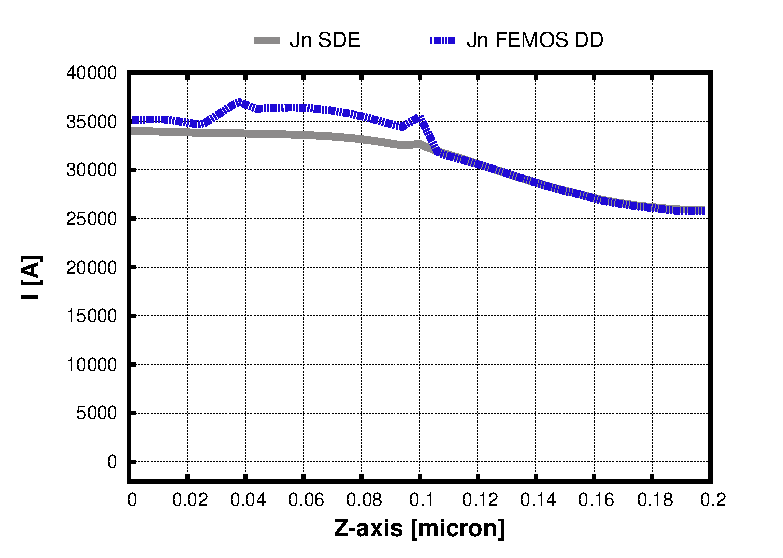
\includegraphics[width = 0.5\textwidth , height=4.5cm]{Corrente/ConfrontiCorrentiBulkJN_SDEVsDD.eps}}
\subfloat[][\emph{Standard DD - Jp}\label{fig: Jp DD}]
{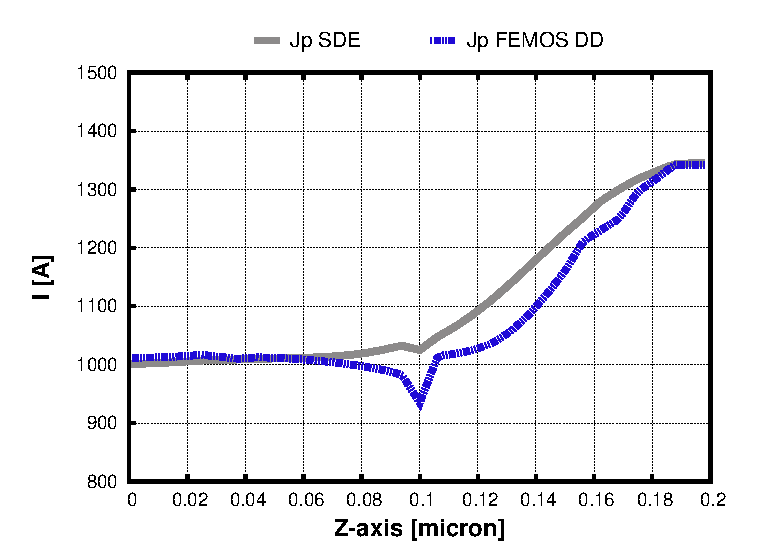
\includegraphics[width = 0.5\textwidth , height=4.5cm]{Corrente/ConfrontiCorrentiBulkJP_SDEVsDD.eps}}


\subfloat[][\emph{SG 3D - Jn}\label{fig: Jn SG 3D}]
{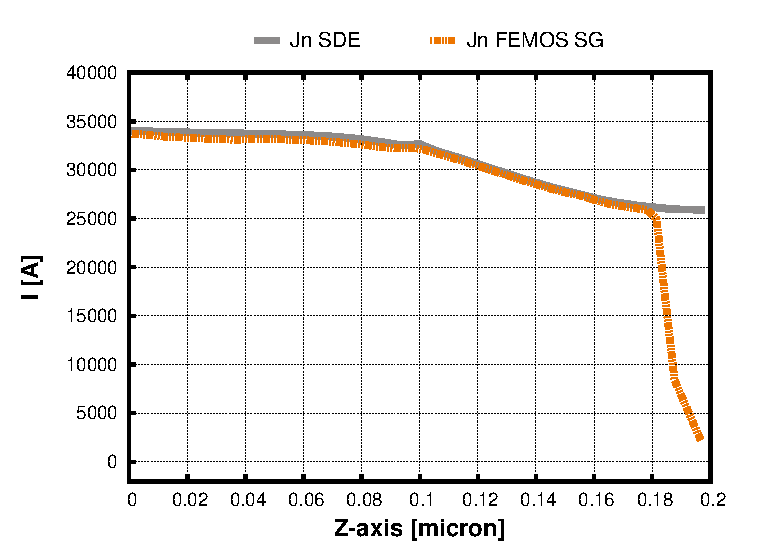
\includegraphics[width = 0.5\textwidth , height=4.5cm]{Corrente/ConfrontiCorrentiBulkJN_SDEVsSG.eps}}
\subfloat[][\emph{SG 3D - Jp}\label{fig: Jp SG 3D}]
{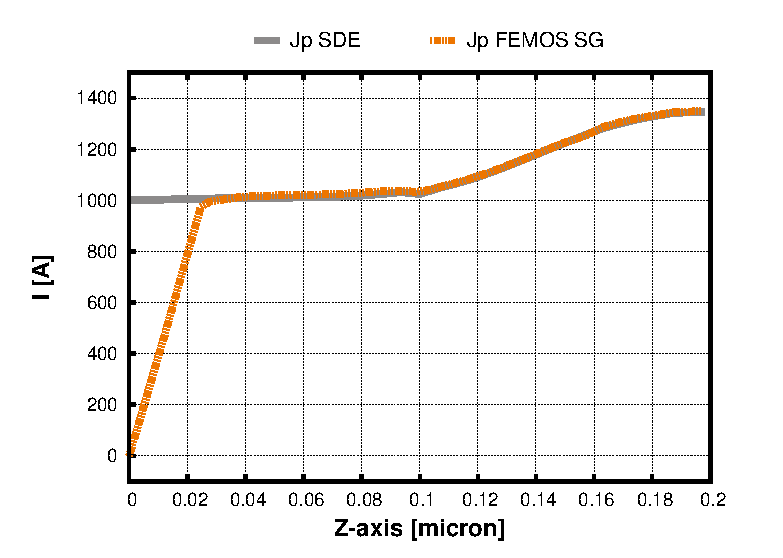
\includegraphics[width = 0.5\textwidth , height=4.5cm]{Corrente/ConfrontiCorrentiBulkJP_SDEVsSG.eps}}

\subfloat[][\emph{Modified DD - Jn}\label{fig: Jn DD mod}]
{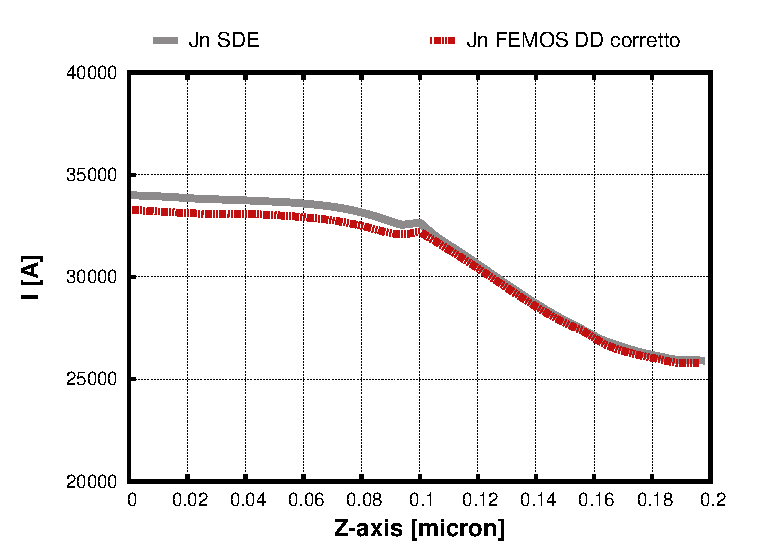
\includegraphics[width = 0.5\textwidth , height=4.5cm]{Corrente/ConfrontiCorrentiBulkJN_SDEVsDDcorretto.eps}}
\subfloat[][\emph{Modified DD - Jp}\label{fig: Jp DD mod}]
{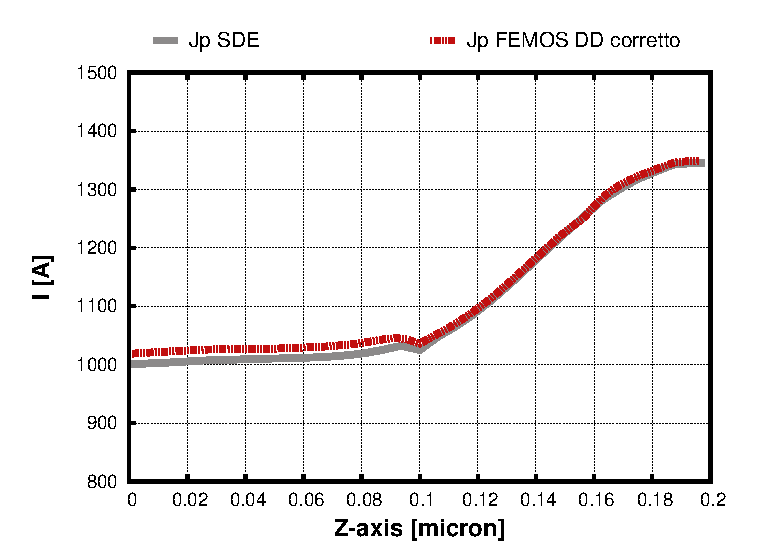
\includegraphics[width = 0.5\textwidth , height=4.5cm]{Corrente/ConfrontiCorrentiBulkJP_SDEVsDDcorretto.eps}}

\caption{1D plot p-n junction - $V_A=1.0[V]$ }
\label{fig: pn current density 1V}
\end{figure}


\begin{figure}[!h]
\centering
\subfloat[][\emph{Hole quasi Fermi potential.}\label{fig: QF hole}]
{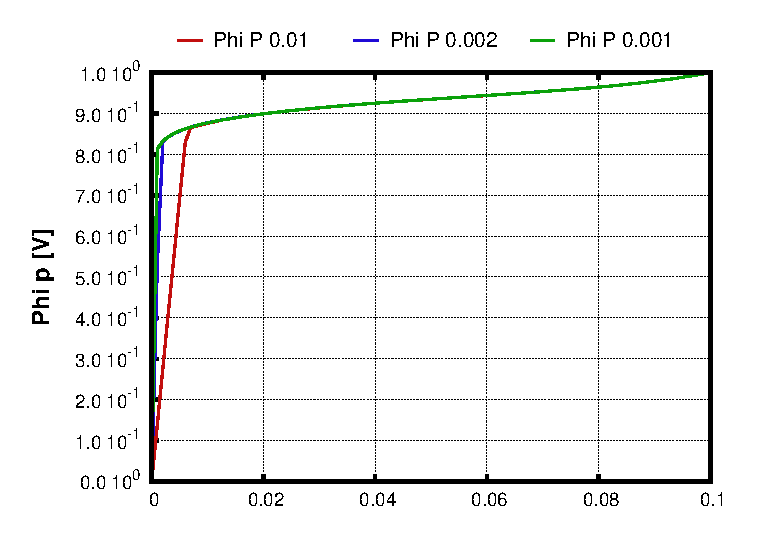
\includegraphics[width = 0.7\textwidth , height=6.5cm]{DatiImmaginiTESI/Diode/ContactFinerQFP.eps}}
\vspace{1cm}
\subfloat[][\emph{Jp.}\label{fig: Jp SG 3D finer}]
{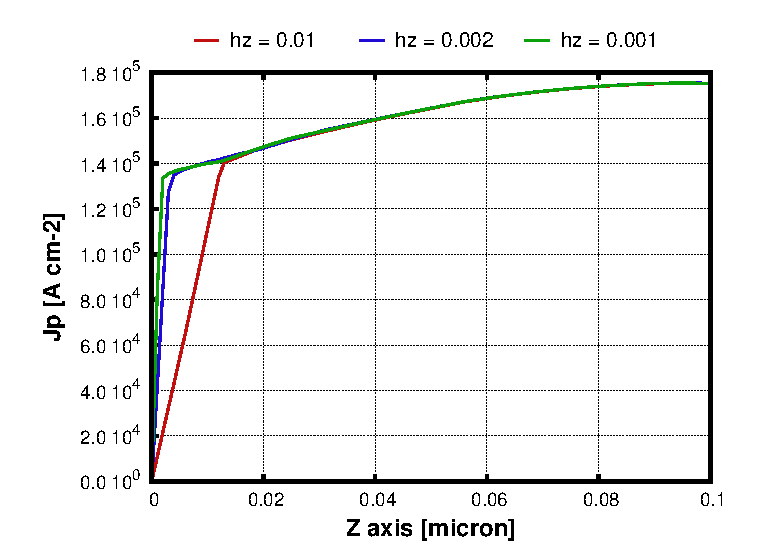
\includegraphics[width=0.7\textwidth , height=6.5cm]{DatiImmaginiTESI/Diode/ContactFinerJP.eps}}

\caption{p-n junction forward biased - mesh refinement at contact}
\label{fig: pn junct mesh refinement}
\end{figure} 



%\begin{figure}[!h]
%\centering
%\subfloat[][\emph{FEMOS}]
%{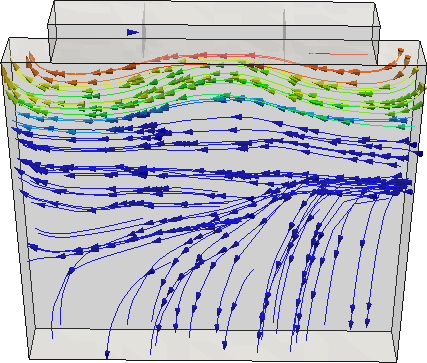
\includegraphics[scale=0.38]{Results/MOS/FEMOS181718_Jn2voltONLYDEVICE.png}}
%\hspace{0.5cm}
%\subfloat[][]
%{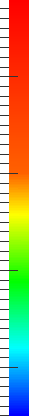
\includegraphics[scale=0.3]{Results/MOS/LegendaArcobalenoVert.png}}
%\hspace{0.5cm}
%\subfloat[][\emph{SDEVICE}]
%{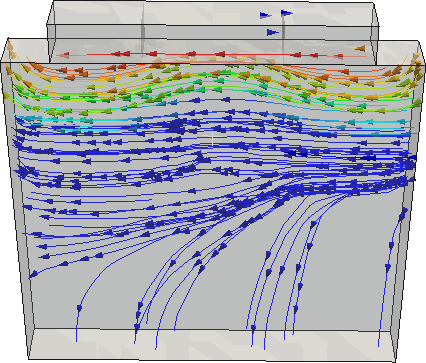
\includegraphics[scale=0.38]{Results/MOS/SDEVICE181718_Jn2voltONLYDEVICE.png}}
%\caption{Electron current density Vgate = 2.0 [V].}
%\end{figure}


%When $(\varphi_{max}-\varphi_{min})$ is small or when the diode is in high direct polarization the modified technique works (\figref{fig: p-n upwinding tech}) better than the Drift-Diffusion formula (\figref{fig: p-n drift diffusion}).
%
%\begin{figure}[!h]
%\centering
%\subfloat[][\emph{Jn}]
%{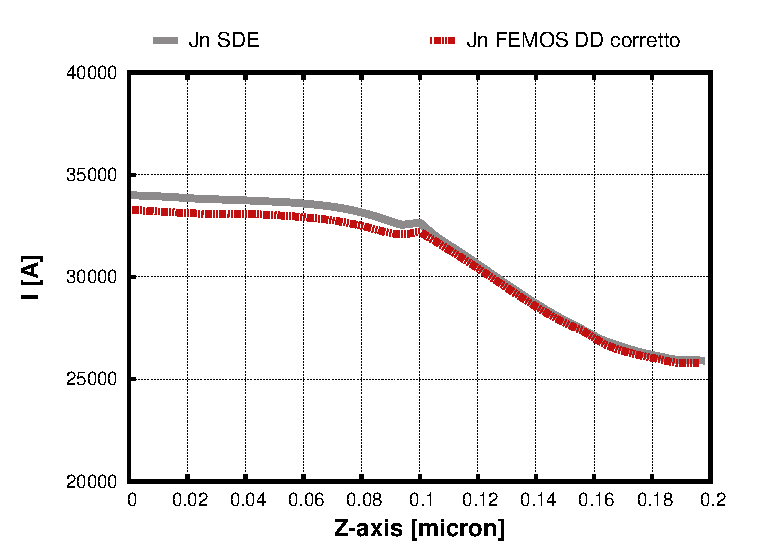
\includegraphics[width = 0.5\textwidth , height=4.5cm]{Corrente/ConfrontiCorrentiBulkJN_SDEVsDDcorretto.eps}}
%\subfloat[][\emph{Jp}]
%{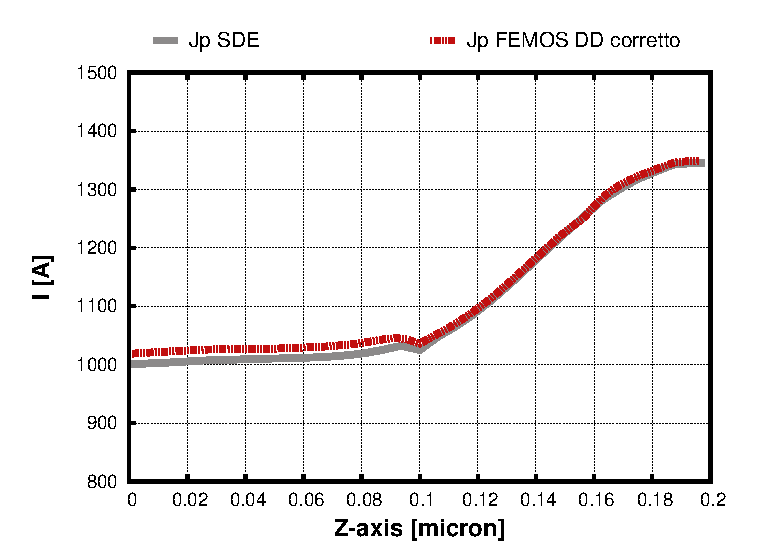
\includegraphics[width = 0.5\textwidth , height=4.5cm]{Corrente/ConfrontiCorrentiBulkJP_SDEVsDDcorretto.eps}}
%\caption{1D plot p-n junction - $V_A=1.0[V]$.}
%\label{fig: p-n upwinding tech}
%\end{figure} 
%
%\begin{figure}[!h]
%\centering
%\subfloat[][\emph{Jn}]
%{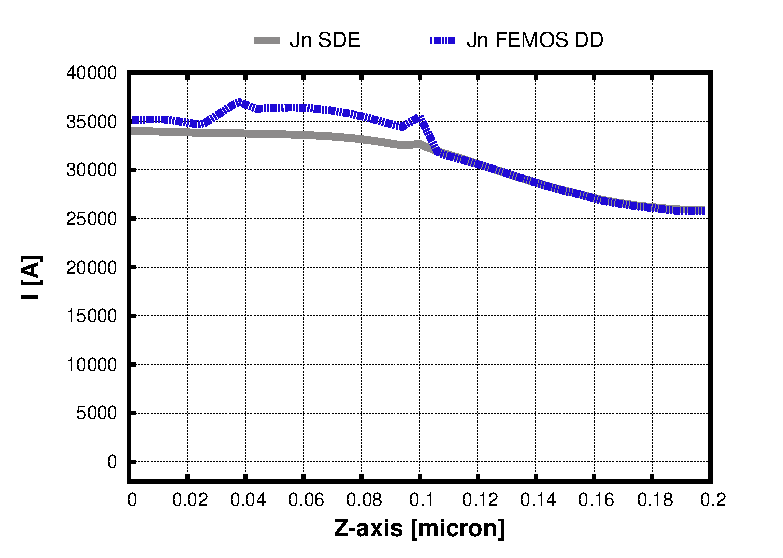
\includegraphics[width = 0.5\textwidth , height=4.5cm]{Corrente/ConfrontiCorrentiBulkJN_SDEVsDD.eps}}
%\subfloat[][\emph{Jp}]
%{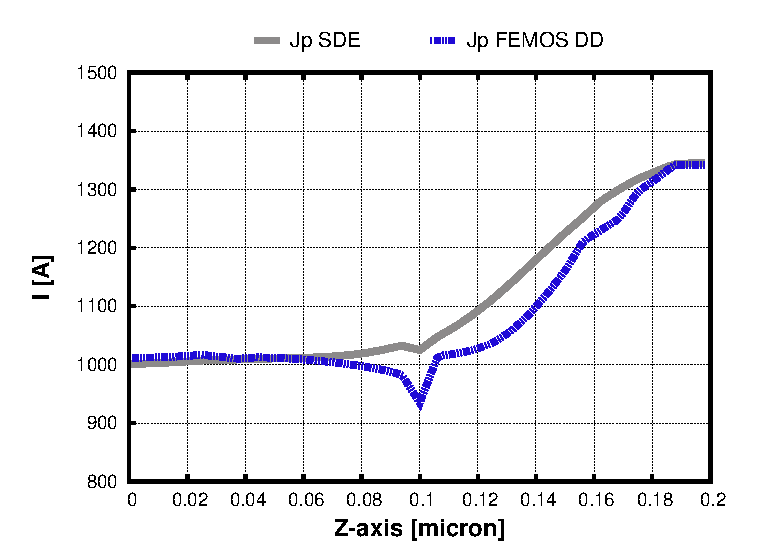
\includegraphics[width = 0.5\textwidth , height=4.5cm]{Corrente/ConfrontiCorrentiBulkJP_SDEVsDD.eps}}
%\caption{1D plot p-n junction - $V_A=1.0[V]$.}
%\label{fig: p-n drift diffusion}
%\end{figure} 





\begin{figure}[!h]
\centering

\subfloat[][\emph{SDE}\label{fig: SDE n-MOSFET Jn}]
{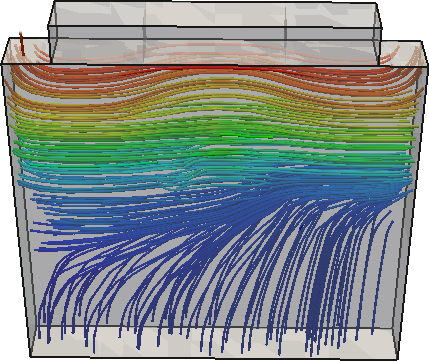
\includegraphics[width = 0.45\textwidth , height=5cm]{CapitoloCorrente/nMOS_SDE.png}}
\hspace{0.1\textwidth}
{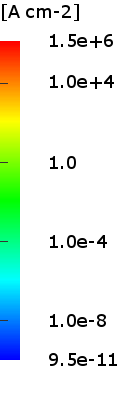
\includegraphics[width = 0.12\textwidth , height=5cm]{CapitoloCorrente/LegendnMOS.png}}



\vspace{1cm}

\subfloat[][\emph{SG} \label{fig: SG 3D scheme nMOS}]
{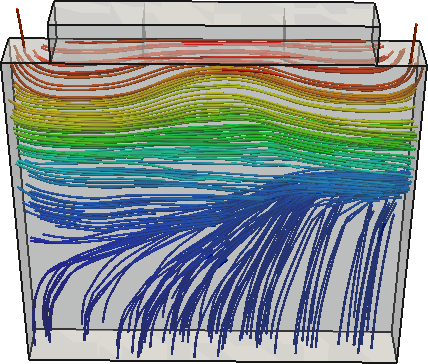
\includegraphics[width = 0.45\textwidth , height=5cm]{CapitoloCorrente/nMOS_SG_device.png}}
\hspace{0.05\textwidth}
\subfloat[][\emph{DD upwind}\label{fig: DD upwind}]
{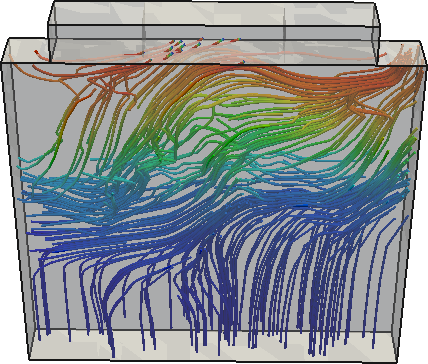
\includegraphics[width = 0.45\textwidth , height=5cm]{CapitoloCorrente/nMOS_DDcorretto.png}}

\vspace{1cm}

\subfloat[][\emph{DD upwind (mesh finer)}\label{fig: DD upwind finer}]
{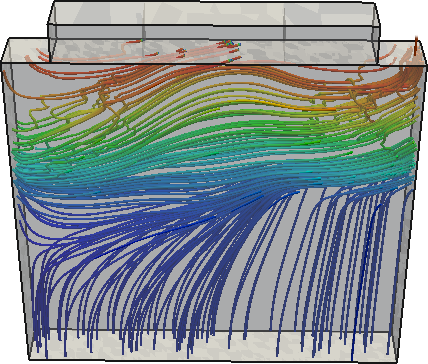
\includegraphics[width = 0.45\textwidth , height=5cm]{CapitoloCorrente/nMOS_DDcorretto35000.png}}
\hspace{0.05\textwidth}
\subfloat[][\emph{DD standard (mesh finer)}\label{fig: DD standard nMOS}]
{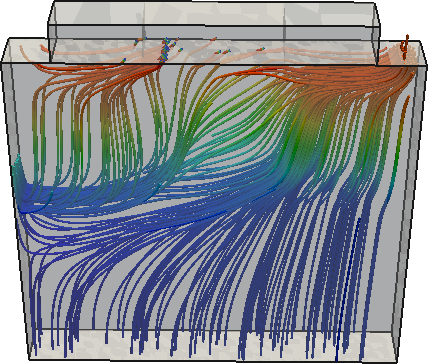
\includegraphics[width = 0.45\textwidth , height=5cm]{CapitoloCorrente/nMOS_DD35000.png}}


\caption{n-MOSFET on-state - $J_n$.}
\label{fig: nMOSFET current methods}
\end{figure} 